\chapter{Additional Simulation Results}
\label{app:sim_results}

This appendix gives the tables and figures of E4 and E5 whose key values
Chapter~\ref{chp:results} states in the text. All runs use HM 0.7 as discovered
with the stop guard; the sources are listed in Appendix~\ref{app:model_inspection}.

\section{Measures and Configurations of E4}

Table~\ref{tab:exp_e4_measures} lists the measures of operational validity and
Table~\ref{tab:exp_e4_configs} the configurations of E4
(Section~\ref{sec:exp_e4_design}).

\begin{table}[htbp]
\centering
\footnotesize
\begin{tabularx}{\textwidth}{L{2.6cm}YL{3.4cm}}
\toprule
\textbf{Perspective} & \textbf{Measures} & \textbf{Why} \\
\midrule
P1 Turnaround time & TTT median, P90 and mean, cycle-time distance (CTD, the Wasserstein-1 or earth mover's distance between the TTT distributions, in minutes), median TTT by flow type & The KPI of the thesis \cite{Chapela2025SimQuality}. \\
P2 Where the time is spent & Mean approach (Gate In to first stop), stop time, transfer between stops and exit, whose four means add up to the mean TTT & Locates the error in the visit. \\
P3 Physical constraints & Trucks in the terminal; share of RMG stops at the busiest block and correlation of block shares with the observed ones; share of RMG stops that start with three or more other trucks at the block; largest number of trucks at one block at once; visits without stop, overlapping stops, visits with more stops than planned & The constraints that the title refers to. \\
P4 Response to load & Spearman correlation of hourly arrivals and hourly median TTT; median TTT by trucks in the terminal; median approach to an RMG first stop by the trucks at that block at Gate In; median RMG stop duration by the other trucks at the block at its start; share of delay-peak hours & The property that E5 needs. \\
Standard BPS measures & 3-gram distance of the activity sequences (NGD-3) and case-arrival distance (CAR) & Comparability with the ProSiT evaluation \cite{Vinci2026prosit,Chapela2025SimQuality}. \\
\bottomrule
\end{tabularx}
\par\smallskip{\footnotesize\raggedright For each load profile in P4, the profile gap is the mean absolute difference between the simulated and the observed medians over the bins.\par}
\caption{Measures of operational validity in E4.}
\label{tab:exp_e4_measures}
\end{table}

\begin{table}[p]
\centering
\scriptsize
\begin{tabularx}{\textwidth}{lL{1.5cm}L{1.6cm}L{1.6cm}L{1.6cm}L{1.3cm}Y}
\toprule
\textbf{Run} & \textbf{Demand} & \textbf{Blocks} & \textbf{Capacity} & \textbf{Waiting} & \textbf{Service} & \textbf{Question} \\
\midrule
\multicolumn{7}{l}{\textit{E4a Demand}} \\
a0 & ProSiT tree & learned & 3, enabling & ProSiT & ProSiT & E3 baseline \\
a1 & hour of week & learned & 3, enabling & ProSiT & ProSiT & Does a realistic arrival profile help? \\
a2 & replay & learned & 3, enabling & ProSiT & ProSiT & Error without demand error \\
\multicolumn{7}{l}{\textit{E4b Block allocation}} \\
b1 & replay & learned, no self-count & 3, enabling & ProSiT & ProSiT & Is the self-count the cause of the concentration? \\
b2 & replay & training shares & 3, enabling & ProSiT & ProSiT & Load-independent allocation \\
b3 & replay & observed & 3, enabling & ProSiT & ProSiT & Blocks from the log where available \\
\multicolumn{7}{l}{\textit{E4c Queue at the block}} \\
c1 & replay & observed & 3, start & ProSiT & ProSiT & Capacity over the whole stop \\
c2 & replay & observed & 3, start & no self-count & ProSiT & Consistent queue feature \\
c3 & replay & observed & 3, start & lane free & ProSiT & Queue arises in the simulation \\
c4 & replay & observed & 4, start & lane free & ProSiT & Four lanes, as in the log (sensitivity) \\
c5 & replay & observed & none & whole delay & ProSiT & Queue learned from data (sensitivity) \\
\multicolumn{7}{l}{\textit{E4d Service under load}} \\
d3--d5 & \multicolumn{4}{l}{as c3--c5} & with load & Does load-dependent service reproduce the stop durations? \\
\multicolumn{7}{l}{\textit{E4e Final configuration (chosen by the rule below)}} \\
e-- & \multicolumn{5}{l}{each change of the final configuration reversed alone} & Is every change needed? \\
eblk & \multicolumn{5}{l}{final configuration with training shares or a learned block choice} & What is lost without the observed blocks? \\
e$\times$ & \multicolumn{5}{l}{final configuration with arrivals compressed or stretched (intensity 0.8, 1.2)} & Does TTT rise with load? \\
eG & \multicolumn{5}{l}{final mechanisms with hour-of-week or ProSiT arrivals and training block shares} & Fully generative accuracy \\
enet & \multicolumn{5}{l}{final configuration with each net of the E3 contrasts} & Does the net matter once queue and service are corrected? \\
\multicolumn{7}{l}{\textit{E4f Training period (in-sample)}} \\
T & \multicolumn{5}{l}{the admissible c1x--c3x and d3x on the training period (replay of the training visits)} & Selection of the final configuration \\
f0 & \multicolumn{5}{l}{final configuration on the training period} & Model error or change between periods? \\
\bottomrule
\end{tabularx}
\par\smallskip{\footnotesize\raggedright ProSiT means the parameter as fitted in E3. No self-count means retrained without counting the stop in its own queue. Lane free means waiting measured from the moment a lane became free. Whole delay means waiting measured from enabling to start. Every configuration from b3 on, and the baseline a0, is also run with an exact count of the activities in progress (suffix x).\par}
\caption{Configurations of E4.}
\label{tab:exp_e4_configs}
\end{table}

\FloatBarrier
\section{Choice and Necessity of the Changes}

Table~\ref{tab:rq2_selection} shows the choice of the final configuration on the
training period (Section~\ref{sec:res_e4_selection}). Table~\ref{tab:rq2_loo}
reverses each change of the final configuration alone and adds the runs with other
block allocations, other arrival intensities and without replay.

\begin{table}[htbp]
\centering
\footnotesize
\begin{tabular}{lcrrrrr}
\toprule
\textbf{Configuration (training period)} & \textbf{Admissible} & \textbf{G-appr.} & \textbf{G-stop} & \textbf{G-WIP} & \textbf{Sum} & \textbf{CTD} \\
\midrule
c1x capacity at start & yes (max 3) & 4.9 & 3.0 & 3.7 & 11.6 & 8.9 \\
c2x + waiting queue without self-count & yes (max 3) & 4.8 & 3.0 & 3.5 & 11.3 & 8.6 \\
c3x lane-free waiting & yes (max 3) & 1.1 & 3.0 & 3.8 & 7.9 & 3.7 \\
d3x = c3x + load-dependent service $\leftarrow$ & yes (max 3) & 0.8 & 1.3 & 3.1 & 5.2 & 4.3 \\
\bottomrule
\end{tabular}
\caption{Choice of the final configuration on the training period (E4f): replayed training visits with their observed blocks, compared with the training log, means over five seeds. Admissible: no rule violation and at most three trucks at a block at once. The configuration with the smallest sum of the profile gaps is chosen ($\leftarrow$). Gaps and CTD in minutes.}
\label{tab:rq2_selection}
\end{table}

\begin{table}[htbp]
\centering
\scriptsize
\setlength{\tabcolsep}{2.4pt}
\begin{tabular}{lrrrrrrrrrrr}
\toprule
\textbf{Configuration} & \textbf{Med.} & \textbf{P90} & \textbf{CTD} & \textbf{Appr.} & \textbf{Stops} & \textbf{Top bl.} & \textbf{Max} & \textbf{Spear.} & \textbf{G-appr.} & \textbf{G-stop} & \textbf{G-WIP} \\
\midrule
Observed (test log) & 33 & 75 & 0.0 & 12.7 & 14.4 & 6.3 & 4 & 0.55 & 0.0 & 0.0 & 0.0 \\
\midrule
\multicolumn{12}{l}{\textit{Final configuration}} \\
d3x = c3x + load-dependent service & 28 & 56 & 7.9 & 10.9 & 10.7 & 6.1 & 3 & 0.54 & 1.1 & 1.3 & 5.9 \\
\midrule
\multicolumn{12}{l}{\textit{One change reversed}} \\
ProSiT count & 27 & 54 & 8.4 & 11.2 & 9.9 & 6.0 & 3 & 0.40 & 1.9 & 2.0 & 7.2 \\
capacity at enabling & 27 & 52 & 9.6 & 9.6 & 10.5 & 5.9 & 10 & 0.46 & 3.8 & 2.7 & 5.9 \\
single-server waiting & 24 & 47 & 13.4 & 5.1 & 11.6 & 6.0 & 3 & 0.14 & 4.9 & 1.1 & 5.8 \\
service without load & 29 & 57 & 7.5 & 10.3 & 11.8 & 6.0 & 3 & 0.44 & 1.6 & 3.0 & 7.3 \\
\midrule
\multicolumn{12}{l}{\textit{Block allocation instead of the observed blocks}} \\
blocks: training shares & 28 & 53 & 9.0 & 10.1 & 10.6 & 6.1 & 3 & 0.48 & 1.6 & 1.3 & 7.3 \\
blocks: learned, no self-count & 28 & 53 & 9.1 & 9.9 & 10.6 & 5.9 & 3 & 0.49 & 1.5 & 1.3 & 6.7 \\
\midrule
\multicolumn{12}{l}{\textit{Arrival intensity (extreme condition)}} \\
arrival intensity 0.8 & 26 & 50 & 10.8 & 8.6 & 10.6 & 6.0 & 3 & 0.40 & 2.0 & 1.3 & 3.2 \\
arrival intensity 1.2 & 33 & 73 & 1.3 & 15.1 & 12.0 & 6.0 & 3 & 0.79 & 1.9 & 1.3 & 5.1 \\
\midrule
\multicolumn{12}{l}{\textit{Fully generative (no replay; training block shares)}} \\
hour-of-week arrivals & 26 & 49 & 11.3 & 8.6 & 10.2 & 6.1 & 3 & 0.47 & 2.1 & 1.3 & 3.8 \\
ProSiT arrivals & 25 & 45 & 13.1 & 7.4 & 9.6 & 6.0 & 3 & 0.08 & 2.5 & 1.3 & 2.5 \\
\midrule
\multicolumn{12}{l}{\textit{First day of the test period}} \\
Observed (13 April) & 49 & 96 & 0.0 & 18.4 & 14.4 & 7.5 & 4 & 0.34 & 0.0 & 0.0 & 0.0 \\
final configuration$^{*}$ & 30 & 65 & 19.0 & 13.9 & 10.8 & 6.5 & 3 & 0.59 & 2.1 & 1.1 & 11.8 \\
blocks: learned (ProSiT)$^{*}$ & 3{,}097 & 7{,}682 & 3{,}368 & 3{,}055 & 15.1 & 100 & 3 & -0.46 & 2{,}880 & 1.0 & 1{,}144 \\
\bottomrule
\end{tabular}
\caption{Final configuration with each change reversed alone, with other block allocations, other arrival intensities and without replay (E4e), against the test log, means over five seeds. $^{*}$Only the 2,393 visits of the first day, because the queue of the learned block choice grows without bound. Med., P90: median and P90 of the TTT; CTD: cycle-time distance; Appr., Stops: mean approach and stop time per visit (all in minutes). Top bl.: share of the RMG stops at the busiest block in \%. Max: largest number of trucks at one block at once in any seed. Spear.: Spearman correlation of hourly arrivals and hourly median TTT. G-appr., G-stop, G-WIP: profile gaps for the approach by trucks at the block, the RMG stop duration by other trucks at the block and the TTT by trucks in the terminal (minutes).}
\label{tab:rq2_loo}
\end{table}


\FloatBarrier
\section{The Final Configuration Against the Observed Logs}

Figure~\ref{fig:sim_ttt_distribution} shows the distribution of the turnaround
time and Figure~\ref{fig:sim_ttt_decomposition} where the time of a visit is spent
(Section~\ref{sec:res_e4_remaining}).

\begin{figure}[htbp]
\centering
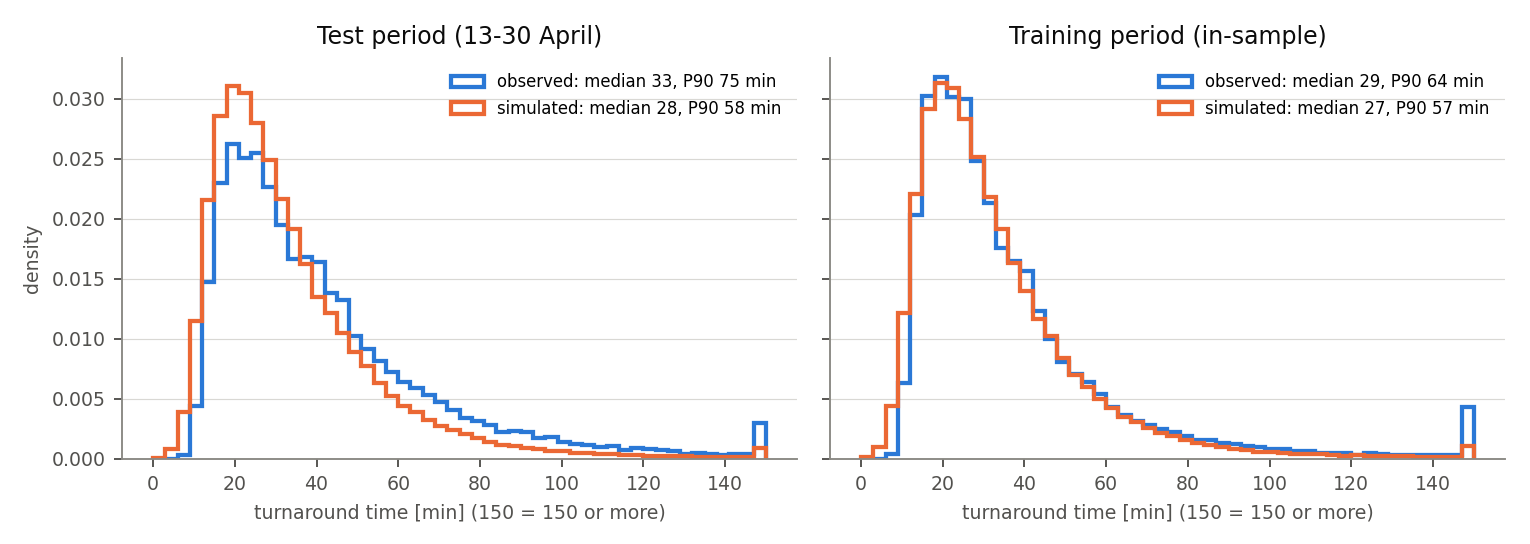
\includegraphics[width=\textwidth]{figures/simulation_model/sim_ttt_distribution.png}
\caption{Turnaround time, observed and simulated with the final configuration (five seeds pooled).}
\label{fig:sim_ttt_distribution}
\end{figure}

\begin{figure}[htbp]
\centering
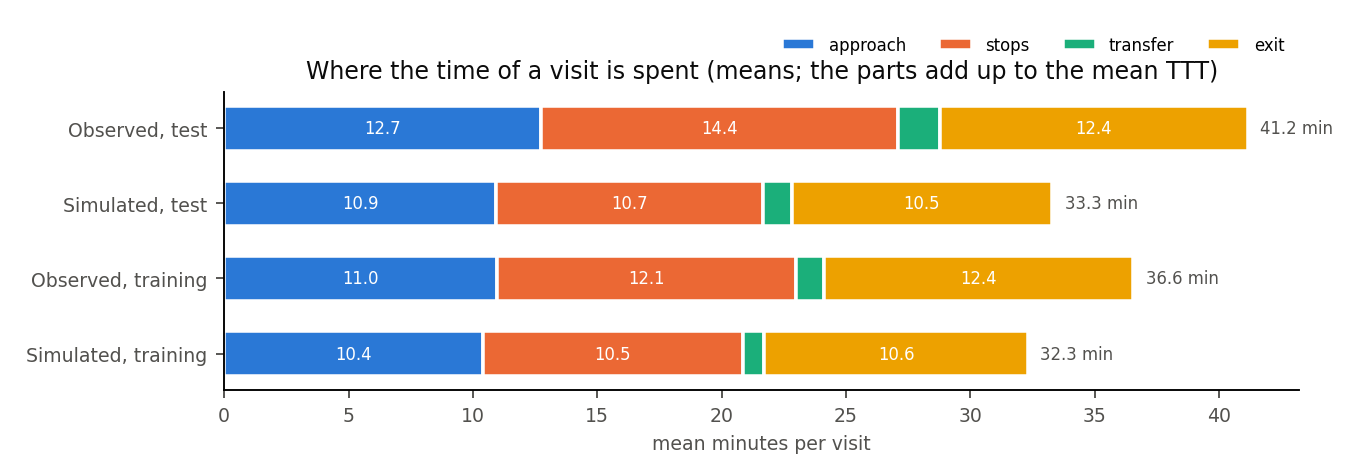
\includegraphics[width=\textwidth]{figures/simulation_model/sim_ttt_decomposition.png}
\caption{Parts of the turnaround time, observed and simulated (means).}
\label{fig:sim_ttt_decomposition}
\end{figure}


\FloatBarrier
\section{Further Results of S1}
\label{app:s1_results}

Table~\ref{tab:rq3_grid_visits} gives the effect of S1 per visit for the six
scenarios of the grid, and Table~\ref{tab:rq3_robustness} the $\pm 2$ variant under
the robustness runs and the design checks (Section~\ref{sec:res_policy}).

\begin{table}[htbp]
\centering
\scriptsize
\setlength{\tabcolsep}{3pt}
\begin{tabularx}{\textwidth}{L{2.6cm}YYYYYY}
\toprule
\textbf{Scenario} & \textbf{Baseline above 35\,min [\%]} & \textbf{Above 35\,min [pp]} & \textbf{In the corridor [pp]} & \textbf{Minutes above 35 per visit} & \textbf{Median TTT [min]} & \textbf{P90 TTT [min]} \\
\midrule
\multicolumn{7}{l}{\textit{Replayed demand of the test period}} \\
S1 $\pm 1$ & 33.5 & $-$2.5\newline [$-$2.9, $-$2.1] & 0.2\newline [$-$0.2, 0.6] & $-$0.95\newline [$-$1.23, $-$0.67] & $-$1.0\newline [$-$1.3, $-$0.7] & $-$2.8\newline [$-$3.7, $-$1.9] \\
S1 $\pm 2$ & 33.5 & $-$3.1\newline [$-$3.7, $-$2.6] & 0.2\newline [$-$0.1, 0.4] & $-$1.11\newline [$-$1.51, $-$0.71] & $-$1.3\newline [$-$1.8, $-$0.8] & $-$3.1\newline [$-$4.3, $-$1.9] \\
S1 any block & 33.5 & $-$3.9\newline [$-$4.4, $-$3.3] & 0.0\newline [$-$0.3, 0.3] & $-$1.41\newline [$-$1.75, $-$1.08] & $-$1.8\newline [$-$2.1, $-$1.5] & $-$4.1\newline [$-$5.2, $-$3.0] \\
\multicolumn{7}{l}{\textit{20\,\% more trucks}} \\
S1 $\pm 1$ & 47.3 & $-$3.6\newline [$-$5.2, $-$2.1] & 1.0\newline [0.5, 1.4] & $-$2.50\newline [$-$5.22, 0.23] & $-$1.8\newline [$-$2.7, $-$0.9] & $-$7.7\newline [$-$14.4, $-$1.0] \\
S1 $\pm 2$ & 47.3 & $-$2.6\newline [$-$4.3, $-$0.8] & 0.6\newline [$-$0.1, 1.2] & 0.57\newline [$-$2.83, 3.98] & $-$1.2\newline [$-$2.0, $-$0.4] & 0.2\newline [$-$9.7, 10.1] \\
S1 any block & 47.3 & $-$4.7\newline [$-$6.3, $-$3.2] & 0.8\newline [0.2, 1.5] & $-$0.23\newline [$-$3.09, 2.63] & $-$2.3\newline [$-$3.3, $-$1.3] & $-$3.4\newline [$-$11.5, 4.7] \\
\bottomrule
\end{tabularx}
\par\smallskip{\footnotesize\raggedright Changes per visit, means over ten paired seeds with 95\,\% $t$-intervals. Minutes above 35 per visit are the mean of $\max(\mathrm{TTT}-35, 0)$ over all visits. In the observed test log, 46.6\,\% of the visits take longer than 35 minutes.\par}
\caption{Effect of S1 per visit, by eligible blocks and demand.}
\label{tab:rq3_grid_visits}
\end{table}

\begin{table}[htbp]
\centering
\scriptsize
\setlength{\tabcolsep}{3pt}
\begin{tabular}{lrrrrr}
\toprule
\textbf{Measure} & \textbf{Main run} & \textbf{(a) service without load} & \textbf{(b) stronger slowdown} & \textbf{(c) intensity 1.2} & \textbf{(d) fully generative} \\
\midrule
Visits with a moved delivery (min) & $-$9.3 [$-$9.9, $-$8.8] & $-$6.6 [$-$7.2, $-$6.0] & $-$13.6 [$-$14.2, $-$13.0] & $-$15.8 [$-$16.6, $-$15.0] & $-$11.1 [$-$11.6, $-$10.6] \\
All visits, mean (min) & $-$2.20 [$-$2.52, $-$1.88] & $-$1.54 [$-$1.78, $-$1.31] & $-$4.68 [$-$5.05, $-$4.31] & $-$4.23 [$-$4.81, $-$3.66] & $-$0.85 [$-$1.05, $-$0.65] \\
All visits, P90 (min) & $-$4.8 [$-$5.4, $-$4.2] & $-$3.3 [$-$4.0, $-$2.6] & $-$11.4 [$-$12.4, $-$10.4] & $-$10.5 [$-$12.0, $-$9.0] & $-$1.4 [$-$1.8, $-$1.1] \\
Approach to the first RMG stop (min) & $-$2.50 [$-$2.72, $-$2.27] & $-$2.10 [$-$2.30, $-$1.89] & $-$5.57 [$-$5.89, $-$5.25] & $-$5.51 [$-$5.86, $-$5.15] & $-$0.80 [$-$0.93, $-$0.67] \\
RMG stops at a full block (percentage points) & $-$6.1 [$-$6.5, $-$5.7] & $-$4.9 [$-$5.2, $-$4.6] & $-$10.0 [$-$10.5, $-$9.5] & $-$7.5 [$-$7.9, $-$7.2] & $-$3.7 [$-$4.0, $-$3.4] \\
RMG deliveries moved (\%) & 22.4 & 24.5 & 28.6 & 30.2 & 15.3 \\
Mean TTT of the affected visits in the baseline (min) & 36.1 & 35.7 & 42.4 & 45.7 & 36.4 \\
\bottomrule
\end{tabular}
\caption{Robustness of S1 $\pm 2$ (Z5): each run against its own baseline, mean over ten paired seeds with 95\,\% $t$-interval. (a) execution time without load; (b) the service model sees one more truck whenever another truck is at the block; (c) arrivals compressed to intensity 1.2; (d) hour-of-week arrivals and training block shares; in (d) the affected visits are compared as groups, not per visit.}
\label{tab:rq3_robustness}
\end{table}

\FloatBarrier
